\chapter{System Development}

\section{ Design}

\begin{figure}[h]
\centering 
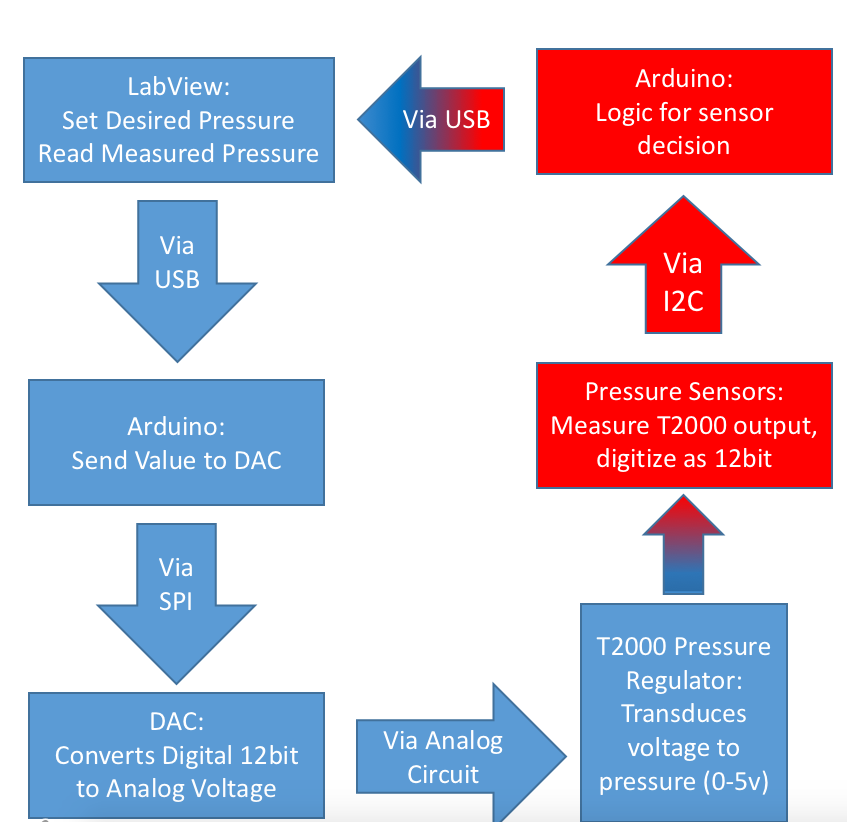
\includegraphics[width=01.0\columnwidth]{PDFCsystemFlowchart.PNG} 
\caption[Communications flowchart for operation of the PDFC]{The control loop used to set and measure channel pressures using the PDFC} 
\label{fig:pneumaticSchematic} 
\end{figure}

\begin{figure}[h]
\centering 
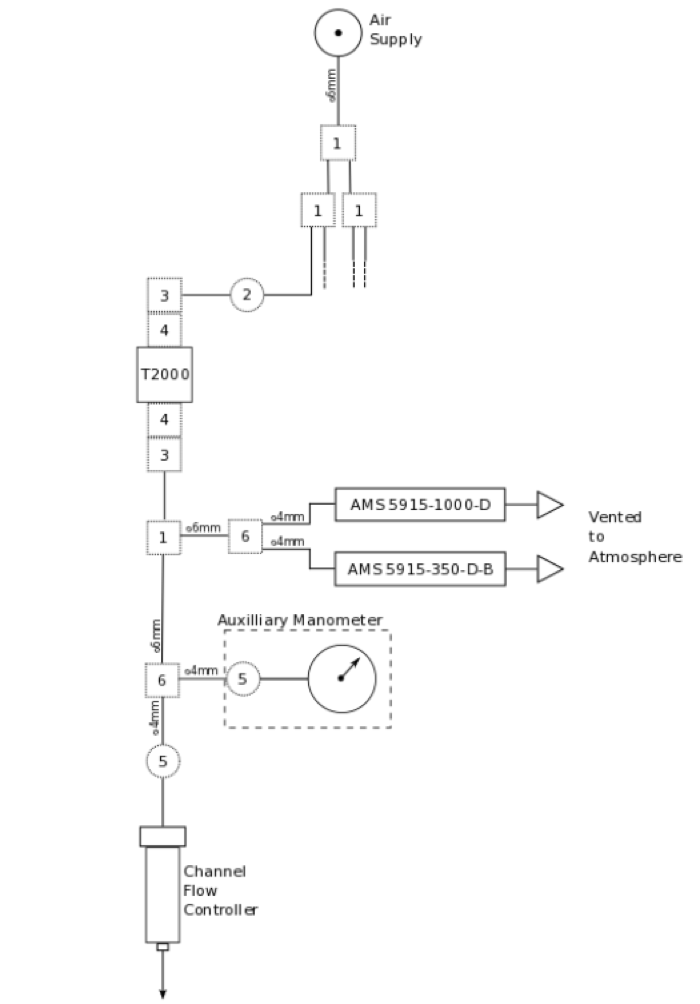
\includegraphics[width=01.0\columnwidth]{pneumaticSchematic.PNG} 
\caption[Pneumatic Schematic of PDFC channel]{The pneumatic schematic detailing a single channel of the PDFC} 
\label{fig:pneumaticSchematic} 
\end{figure}

\section{Characterization}

Note on time response:
"The major drawback of passive control is the slow response
time in the order of seconds or even minutes.32 The long
response time comes from the relatively large fluidic resistance
of the tubing and the fluidic capacitance caused by the
compressibility of the liquid or the channel material.33,34"\cite{Chong2016}

